\documentclass[border=10pt]{standalone}
\usepackage{tikz}
\usetikzlibrary{shapes.geometric, arrows.meta, positioning, calc, shadows, fit, backgrounds}

\begin{document}
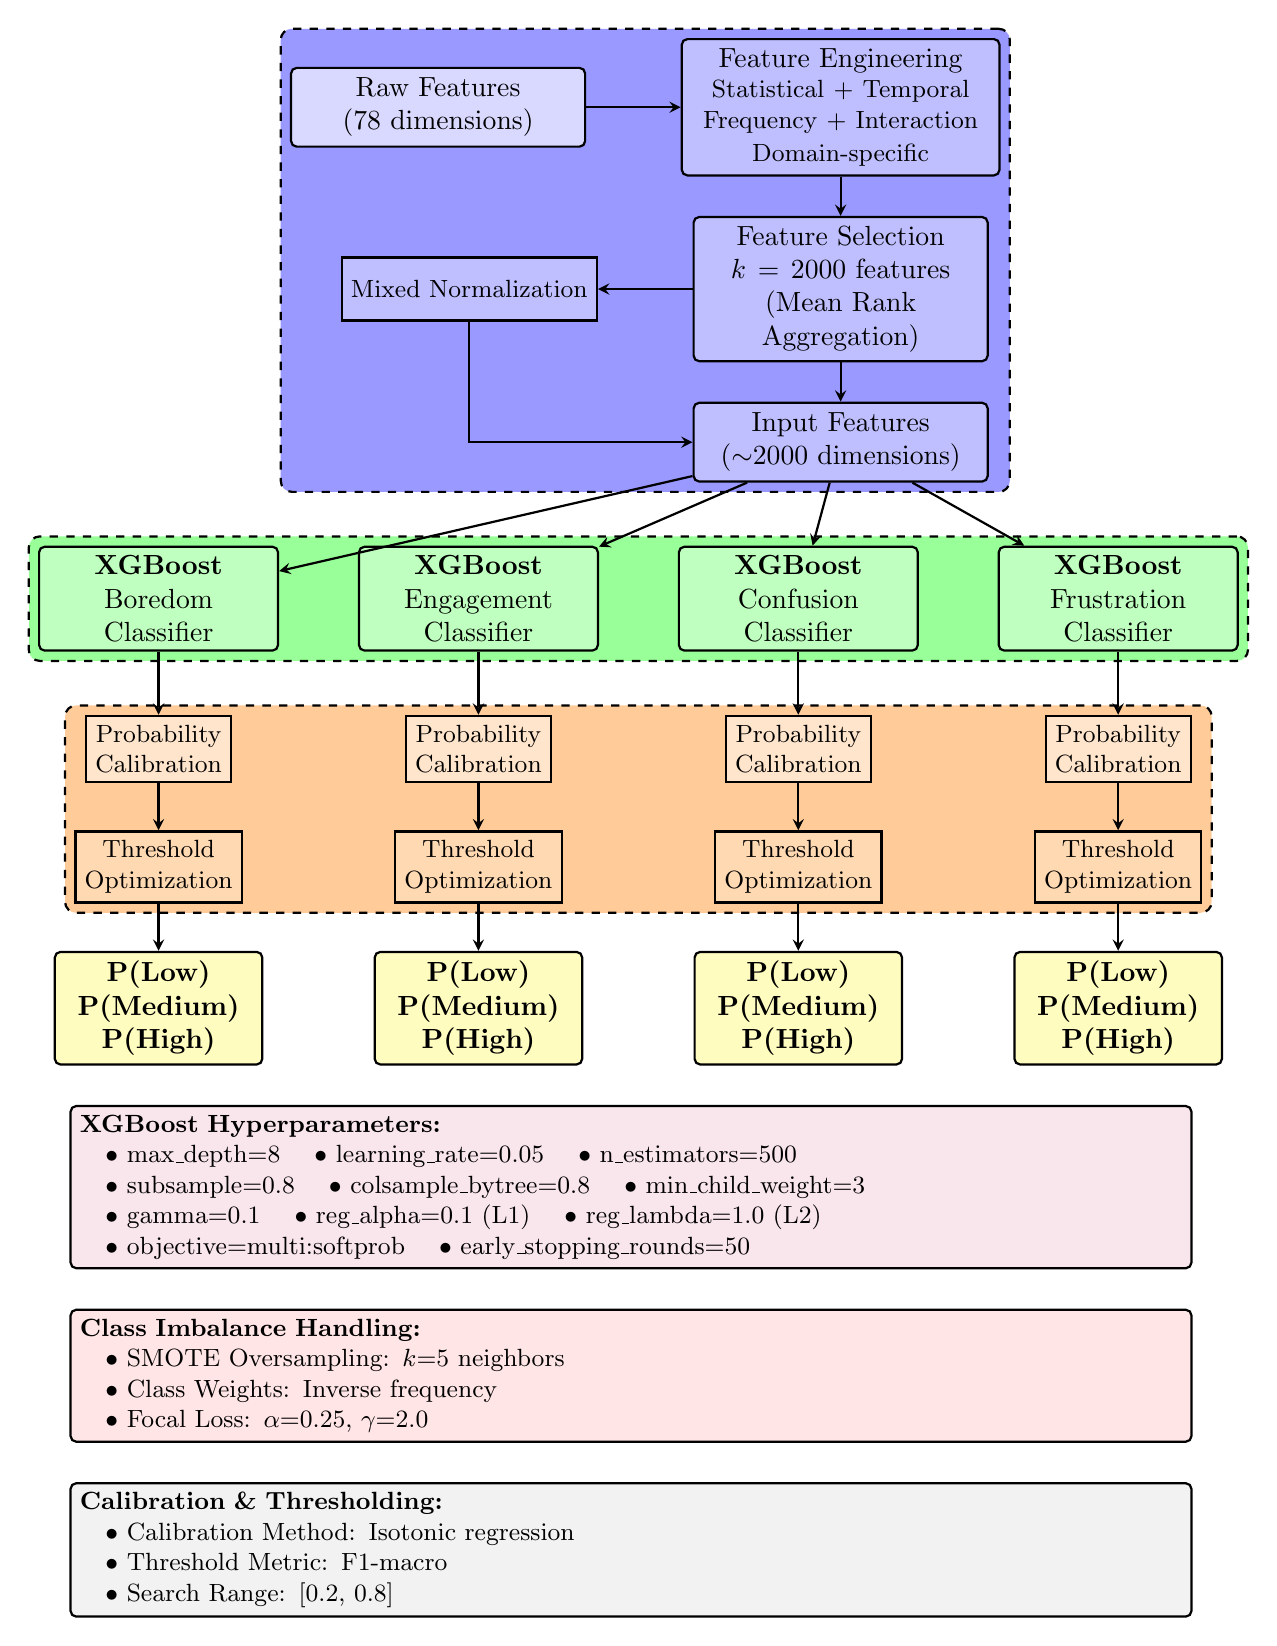
\begin{tikzpicture}[
    node distance=12mm and 8mm,
    box/.style={rectangle, draw, thick, align=center, minimum height=10mm, rounded corners=2pt},
    smallbox/.style={rectangle, draw, thick, align=center, minimum height=8mm, font=\small},
    arrow/.style={->, thick, >=stealth},
    group/.style={draw, dashed, thick, rounded corners, fill opacity=1},
    label/.style={font=\bfseries\small}
  ]

  % ============ INPUT PIPELINE ============
  % Raw Input
  \node[box, fill=blue!15, text width=3.5cm] (raw) {Raw Features\\(78 dimensions)};

  % Feature Engineering
  \node[box, fill=blue!25, right=1.2cm of raw, text width=3.8cm] (feng) {Feature Engineering\\{\small Statistical + Temporal\\Frequency + Interaction\\Domain-specific}};

  % Feature Selection
  \node[box, fill=blue!25, below=0.5cm of feng, text width=3.5cm] (fsel) {Feature Selection\\$k=2000$ features\\(Mean Rank Aggregation)};

  % Normalization
  \node[smallbox, fill=blue!25, left=1.2cm of fsel] (norm) {Mixed Normalization};

  % Input to Models
  \node[box, fill=blue!25, below=0.5cm of fsel, text width=3.5cm] (input) {Input Features\\($\sim$2000 dimensions)};

  % Arrows for preprocessing
  \draw[arrow] (raw) -- (feng);
  \draw[arrow] (feng) -- (fsel);
  \draw[arrow] (fsel) -- (input);
  \draw[arrow] (fsel) -- (norm);
  \draw[arrow] (norm) |- (input);

  % ============ CLASSIFIERS ============
  % 4 XGBoost Classifiers
  \node[box, fill=green!25, below left=0.8cm and 5.25cm of input, text width=2.8cm] (bore) {\textbf{XGBoost}\\Boredom Classifier};
  \node[box, fill=green!25, right=1cm of bore, text width=2.8cm] (enga) {\textbf{XGBoost}\\Engagement Classifier};
  \node[box, fill=green!25, right=1cm of enga, text width=2.8cm] (conf) {\textbf{XGBoost}\\Confusion Classifier};
  \node[box, fill=green!25, right=1cm of conf, text width=2.8cm] (frus) {\textbf{XGBoost}\\Frustration Classifier};

  % Arrows to classifiers
  \draw[arrow] (input) -- (bore);
  \draw[arrow] (input) -- (enga);
  \draw[arrow] (input) -- (conf);
  \draw[arrow] (input) -- (frus);

  % ============ POST-PROCESSING ============
  % Calibration
  \node[smallbox, fill=orange!20, below=0.8cm of bore] (cal1) {Probability\\Calibration};
  \node[smallbox, fill=orange!20, below=0.8cm of enga] (cal2) {Probability\\Calibration};
  \node[smallbox, fill=orange!20, below=0.8cm of conf] (cal3) {Probability\\Calibration};
  \node[smallbox, fill=orange!20, below=0.8cm of frus] (cal4) {Probability\\Calibration};

  \draw[arrow] (bore) -- (cal1);
  \draw[arrow] (enga) -- (cal2);
  \draw[arrow] (conf) -- (cal3);
  \draw[arrow] (frus) -- (cal4);

  % Threshold Optimization
  \node[smallbox, fill=orange!30, below=0.6cm of cal1] (thresh1) {Threshold\\Optimization};
  \node[smallbox, fill=orange!30, below=0.6cm of cal2] (thresh2) {Threshold\\Optimization};
  \node[smallbox, fill=orange!30, below=0.6cm of cal3] (thresh3) {Threshold\\Optimization};
  \node[smallbox, fill=orange!30, below=0.6cm of cal4] (thresh4) {Threshold\\Optimization};

  \draw[arrow] (cal1) -- (thresh1);
  \draw[arrow] (cal2) -- (thresh2);
  \draw[arrow] (cal3) -- (thresh3);
  \draw[arrow] (cal4) -- (thresh4);

  % ============ OUTPUT ============
  % Output nodes - 3 classes (Low, Medium, High)
  \node[box, fill=yellow!25, below=0.6cm of thresh1, text width=2.4cm] (out1) {\textbf{P(Low)}\\\textbf{P(Medium)}\\\textbf{P(High)}};
  \node[box, fill=yellow!25, below=0.6cm of thresh2, text width=2.4cm] (out2) {\textbf{P(Low)}\\\textbf{P(Medium)}\\\textbf{P(High)}};
  \node[box, fill=yellow!25, below=0.6cm of thresh3, text width=2.4cm] (out3) {\textbf{P(Low)}\\\textbf{P(Medium)}\\\textbf{P(High)}};
  \node[box, fill=yellow!25, below=0.6cm of thresh4, text width=2.4cm] (out4) {\textbf{P(Low)}\\\textbf{P(Medium)}\\\textbf{P(High)}};

  \draw[arrow] (thresh1) -- (out1);
  \draw[arrow] (thresh2) -- (out2);
  \draw[arrow] (thresh3) -- (out3);
  \draw[arrow] (thresh4) -- (out4);

  % ============ GROUPS ============
  \begin{scope}[on background layer]
    % Preprocessing group
    \node[group, fill=blue!40, fit=(raw) (feng) (fsel) (norm) (input), label={[label, above=0.2cm]above:Preprocessing Pipeline}] (preproc) {};

    % XGBoost models group
    \node[group, fill=green!40, fit=(bore) (enga) (conf) (frus), label={[label, above=0.1cm]above:4 Independent XGBoost Classifiers}] (xgb) {};

    % Post-processing group
    \node[group, fill=orange!40, fit=(cal1) (cal2) (cal3) (cal4) (thresh1) (thresh2) (thresh3) (thresh4), label={[label, above=0.1cm]above:Post-Processing}] (post) {};
  \end{scope}

  % ============ TRAINING COMPONENTS (below) ============
  \node[box, fill=purple!10, below=0.5cm of out1, xshift=6.0cm, text width=14cm, align=left, font=\small] (params) {
    \textbf{XGBoost Hyperparameters:} \\
    \quad $\bullet$ max\_depth=8 \quad $\bullet$ learning\_rate=0.05 \quad $\bullet$ n\_estimators=500 \\ \quad $\bullet$ subsample=0.8 \quad $\bullet$ colsample\_bytree=0.8 \quad $\bullet$ min\_child\_weight=3 \\
    \quad $\bullet$ gamma=0.1 \quad $\bullet$ reg\_alpha=0.1 (L1) \quad $\bullet$ reg\_lambda=1.0 (L2) \\ \quad $\bullet$ objective=multi:softprob \quad $\bullet$ early\_stopping\_rounds=50
  };

  \node[box, fill=red!10, below=0.5cm of params, text width=14cm, align=left, font=\small] (imbalance) {
    \textbf{Class Imbalance Handling:} \\
    \quad $\bullet$ SMOTE Oversampling: $k$=5 neighbors \\ \quad $\bullet$ Class Weights: Inverse frequency \\ \quad $\bullet$ Focal Loss: $\alpha$=0.25, $\gamma$=2.0
  };

  \node[box, fill=gray!10, below=0.5cm of imbalance, text width=14cm, align=left, font=\small] (misc) {
    \textbf{Calibration \& Thresholding:} \\
    \quad $\bullet$ Calibration Method: Isotonic regression \\ \quad $\bullet$ Threshold Metric: F1-macro \\ \quad $\bullet$ Search Range: [0.2, 0.8]
  };

\end{tikzpicture}
\end{document}
